\documentclass[11pt, openany]{book}              % Book class in 11 points
\parindent0pt  \parskip10pt             % make block paragraphs
\raggedright                            % do not right justify
\usepackage{graphicx}
%\graphicspath{ {./images/} }
\title{\bf Quantitative Investment Handbook}    % Supply information
\author{Xinhe Liu}              %   for the title page.
\date{2018-5-28}                           %   Use current date. 

% Note that book class by default is formatted to be printed back-to-back.
\begin{document}                        % End of preamble, start of text.
% \frontmatter                            % only in book class (roman page #s)
\maketitle                              % Print title page.
\tableofcontents                        % Print table of contents
\mainmatter                             % only in book class (arabic page #s)

\part{Financial Market and Investment Tools}

\chapter{Economics and Econometrics}

\section{Macroeconomics} 

GDP, Inflation and Unemployment:

\begin{itemize}
    \item GDP = C + I + G + X 
    \item CPI, RPI, PPI, Core CPI, Nonfarm Payroll, HICP (Europe)
    \item Philips Curve(Inflation and Unemployment)
    \item Unemployment Rate(labor force), Participation Rate(total population), Quit Rate 
    \item Unemployment: Frictional, Cyclical, Structural, Seasonal, Voluntary 
\end{itemize}

Economic Indicators: \\

Leading Indicators: 

\begin{itemize}
    \item PMI, Tanken Survey(Japan)
    \item Capacity Utilisation 
    \item Retail Sales
    \item Consumer Sentiment/Confidence 
\end{itemize}


Market Data Release Time Schedule:

\begin{center}
 \begin{tabular}{||c c||} 
 \hline
 Time & Market Data \\ [0.5ex] 
 \hline
 Week 1 & Employment Situation (First Friday), ISM \\ 
 Week 2 & Retail Sales, Consumer Sentiment \\ 
 Week 3 & CPI, IP \\ 
 Week 4 & Durable Goods, GDP, Consumer Sentiment(UoM final \& Conference Board) \\ 
 \hline
\end{tabular}
\end{center}

\begin{itemize}
    \item PMI 
    \item Capacity Utilisation 
    \item Retail Sales
    \item Consumer Sentiment/Confidence 
\end{itemize}
Fiscal Policy and Monetary Policy:

\begin{itemize}
	\item General Economic Goals: Full Employment, Economic Growth, Low Inflation
	\item Fiscal Policy: Government Spending and Tax Policy
    \item Monetary Policy: Open Market Operations, Discount Rate, Reserve Requirement, Federal Fund Rate(Upper Limit for Repo Rate) (In other countries: Overnight discount rate, Refi Rate, Deposit Rate, Main Lending Rate) 
    \item Interaction: Crowding Out: Higher Interest Rates may cause investment and consumption 
    \item Central bank, Taylor rule
\end{itemize}

\subsection{Business Cycle and Debt Cycle}

According to Ray Dailo's Opinion, business cycles are created by credit (borrowing). Growth = Productivity Growth + Debt Cycle Effect.  

\begin{itemize}
	\item Total output = Price $\times$ Quantity, while Price = Money + Credit
	\item Long term debt cycle: 75 to 100 years. Short term debt cycle" 5-7 years
	\item Key indicators Inflation, deflation, tax, government spending, unemployment (Government Action)
	\item "Beautify Deleveraging": The phase total debt decreases. Needs: Spending cut, Debt Restructuring, Wealth transfer, Print Money (Government Debt increases, total debt decreases, if not carefully, lead to hyper-inflation
	\item 2-3 years depression/deleveraging and 7-10 yeas "reflation"
\end{itemize}

Keysian Theory 

stagflation and non zero inflation


\section{Financial Economics}
\begin{itemize}
    \item Rationality. Utility Theroy, Indifference Curve, Risk Aversion. Participants are perfect optimizers with perfect Bayesian Information
    \item Efficient Market Hypothesis : 3 Forms
    \item Market Anomalies: Fundamental Anomalies (Factor), Technical Anomalies, Calendar Anomalies, Limits to Arbitrage 
\end{itemize}

\section{Behavioral Finance}

\begin{itemize}
    \item Behavioral Finance micro: Assumes limited information, bounded rationality
    	\subitem Prospect Theory
    	\subitem Neuro-economics
    \item Behavioral Finance macro
\end{itemize}


\chapter{Basic Financial Concepts}                % Print a "chapter" heading

This chapter summarizes some basic financial concepts you should know about.



\section{Asset Management}

Asset Owners(Real Money): From conservative to active: Banks, Insurance Company, Defined Contribution Plan, Pension, Endowment/Foundations 

Hedge Funds(Fast Money)

Investment Purpose Statement(IPS): Consider Return, Risk, Time Horizon, Tax, Liquidity, Legal and Unique. 

\section{Accounting, Corporate Finance and Fundamental Analysis}

Accounting:
\begin{itemize}
    \item Balance Sheet, Income Statement, Cash flow Statement Basics
    \item EBIT = operating profit + non recurring expense - non-recurring income, EBITDA, Operating profit, normalized net income = NI + non recurring items
    \item Gross Profit, Operating profit, profit before tax, net income
    \item Gross Margin, EBIT Margin, EBIT Margin, Net Operating Margin, Net Profit Margin 
    \item Cash flow from Operations = NI + DA +- change in inventory/accounts payable, receivable, operating items
    \item CF from investing = Capital Expenditure -+ Disposal/Purchase of Assets
    \item CF from financing = -Dividend - Share buybacks + issuance of stock/bond
    \item Equity: Preferred shares, authorized shares (maximum shares the board can issue), Treasury stock, buy back book value, Free float Market capitalization = share price * ( shares outstanding - shares not traded), Small free float: little share holder control, volatile share price, high premium in M\&A 
\end{itemize}

Capital Structure:

\begin{itemize}
	\item Operating items vs financing items ( cash, financial asset/liability, equity)
	\item Working Capital = Current Assets - Current Liabilities, Operating Working Capital = Operating Assets - Operating Liabilities(exclude cash)
	\item Inventory COGS LIFO FIFO inventory turnover
	\item Payable days, receivable days, working capital cycle (payable days - inventory days + receivable days)
	\item Leverage ratios: Debt/Equity, Total Debt/EBITDA, EBITDA/inst expense	
\end{itemize}

Credit Scoring/Credit Analysis
\begin{itemize}
    \item Credit Risk = Business Risk( Country, Economic Cycle, Industry Cycle, Currencies, Commodities, trends) + Financial Risk(Cash Risk)
    \item Creditor Cashflow Statement Net Income + D/A/non-cash items = FFO( Funds from Operations), FFO +- Decrease/Increase in OWC = Operating Cash Flow, Operating Cash Flow - Capex = Free Operating Cash Flow(FOCF)\\ FOCF + Dividends = Discretionary Cash Flow, DCF +- Acquisition, Asset Disposals, Net other sources/uses of cash = pre-financing cashflow +- Increase(Decrease) in Debt, +- Net Sale/Repurchase of Shares = Inc/(Dec) in Cash/Securities
    \item Profitability \& Efficiency Ratios: EBIT/EBITDA margin, Return on Assets, Return on Invested Capital
    \item Coverage Ratios: EBITDA/interest(net interest), EBITDA/(interest + Principal Amortization), EBIT/interest or net interest
    \item Leverage Ratios: Debt/Equity, Debt/Capital, Debt/EBITDA
    \item Cash flow adequacy Ratios: FFO/Debt, FOCF/Debt, Free Cash flow/Debt, Retained Cash Flow/Debt
    \item Liquidity Ratios: maturing debt principal this year/FFO or discretionary cash flow, Quick Ratio = (Cash + Marketable Securities + Committed un-used bank credit lines)/maturing debt principal this year.
\end{itemize}

Tax:  Effective Tax Rate, Loss Harvesting and Tax-Aware investment 

Valutaion fundamentals: 

\begin{itemize}
	\item Intrinsic Value and two approaches - absolute valuation and relative valuation 
	\item Enterprise Value = Debt + Equity Value - Cash/Cash Equivalent = Net Debt Value + Equity Value
	\item Equity Value (affected by performance (operating), investing and financing (leverage)) = Price x Shares Outstanding
	\item Asset = Enterprise Value + Non-core assets(not valued by Multiples/DCF models, like cash)
	\item Free Cash Flow Calculation: EBIT - tax on EBIT (LT tax rate x EBIT) = NOPAT (net operating profit after tax )/EBIAT, Free Cash flow = NOPAT + D\&A - capex - increase in OWC + decrease in OWC - Increase in Other net operating assets + Decrease in other net operating assets -+ change in Long term tax liabilities
	\item FCFF, FCFE 
	\item Discount Rate- Weighted Average Cost of Capital (WACC) - CAPM / required rate of return, WACC = D/(D+E) cost of net debt x (1-t) + $(rf+(r_m-r_f)\times beta)\times E/(D+E)$, D is net debt
	\item Gordon Growth Model
	\item EV multipliers : EV/Sales, EV/EBIT,EV/EBITDA
\end{itemize}


Fundamental Analysis, Company Analysis and Value Investing

Management/Strategic Analysis(SWOT, Five forces etc), Industry/Region/ Sector Analysis + competitor Analysis 

\section{ Real-life trading}

\begin{itemize}
    \item Shorting a Stock: achieved by a stock-loan process of broker/dealer: broker need to borrow and put colleteral, during borrow agreement, any dividend is passed (synthetically) from the borrower to the beneficial owner. Corporate actions: borrower vote as in lender's proxy. 
    \item SHOrt squeeze: Stock with high short interest trended upwards, short side cover their shorts.
    \item Naked short: short (t+2) before borrow, can borrow/buy later.
    \item Short interest thredhold: 8\% of market cap or free float.
    \item Prime-brokerage: Agency only brokerage does not own books
\end{itemize}

\chapter{Major Asset Classes and Asset Valuation Theories}
\section{Money Market}

\begin{itemize}
    \item Overnight (O/N) reference ratesL SONIA(Sterling Overnight Index Average), EONIA, SOFR - ALl has different day count convention
    \item LIBOR Rate, STIR Futures (Cash Settlement by 100 - expected interest) , IMM Dates( Exchange for interest rate and currency futures)
    \item T-bill(1,3,6,12 Month) , T-note, T-bond
    \item Commercial Paper( Issued by best quality companies)
    \item Day Count Conventions
    \item Repo Market: Repo(seller, needs cash), Reverse Repo(buyer, owns collateral for a while)
    \item Fed Funds Rate: 
    \begin{itemize}
    	\item The Upper Bound: Interest on Excess Reserves: interest rate paid by the Fed on Excess reserves held by banks at the Fed. (many money market participants are not reserve account holders so they do not have access to the IOER). 
    	\item Lower Bound: Overnight RRP: Non-reserve account holder can earn interest by entering into an overnight reserve repo(overnight RRP)- offer each day.
    \end{itemize}
\end{itemize}

\section{Asset Management Overview}
factor investors

market - CAPM + APT

value - HML
  FX carry trade
  commodity - roll returns
  Fixed Income - riding the yield curve 
  
momentum 
   UMD - up minus down
   WML - winner minus losers

size -SML 


volatility risk premium ( a negative risk premium)
illiquidity risk premium ‘


alpha and active investing


Fundamental Theorem of Active Management


backtesting

  surviorship bias
  sample selection bias
  infrequent trading (report same price/ missing price) 



hedge fund strategies

  merger/risk arbitrage

   fixed income arbitrage
       swap spread arbitrage
       yield-curve spread arbitrage
      mortgage spread arbitrage ( on prepayment rates)
      capital structure/credit arbitrage 
      volatility trading (interest cap vol) arbitrage
\section{FX}

Basic Concepts:
\begin{itemize}
    \item FX Market is Extremely liquid (smaller bid ask spread on equity) 
    \item Market Size High to Low: USD, EUR, Cheap Currencies: JPY(safe currency), CHF, GBP, Rich(high rate) currencies: ZAR, MXN, AUD 
    \item Uncovered Interest Rate Parity and Covered IRP
    \item Interest Rate Forward/Futures, Non-deliverable forwards(NDF)
    \item FX Drivers: Interest rate differential, inflation rate differential, Global M\&A/Capital Flows, Technical Drivers(Indicators), Central Bank Policies, Risk Appetite
    \item Purchasing Power Parity
\end{itemize}

\section{Equity}
Sell Side Services
\begin{itemize}
    \item Traditionally, Sales and Trading Service build around research (content stream)
    \item New Model -automation: Algo-trading, Dark pools, MiFID
    \item ETF Market: Market Maker/Specialist who issue ETF Shares to investors, buy underlying stocks with ETF or money from fund and stock exchange.
    	\subitem Physical ETF: generate return from holding all, or samples of underlying shares like index funds. Kept safe by a custodian.
    	\subitem Synthetic ETF: Entering into total return swaps with counterparty issuer. 
   		\subitem ETFs fo pay dividends monthly, quarterly, half-yearly or annual. Based on funds income net of expense and distribute to share holders on the register on record date. Paid via brokerage account. 
   		\subitem Tracking error: Annual fees are deducted Reflecting daily NAVs. 
\end{itemize}



\section{Currency/Foreign Exchange}
\section{Fixed-Income}
Basic Concepts:
\begin{itemize}
    \item Day Count Convention, Dirty Price
    \item Macaulay Duration, Modified Duration, DV01, Dollar Duration, Effective Duration
    \item Maturity Effect, Coupon Effect, Yield Effect, Coupon Frequency Effect on Duration
    \item Term Structure of Yield Curve, Expectation Theory, Liquidity Preference Hypothesis, Segmented Markets/Preferred Habitat Theory. Bond Markets: < 1 y (money market) 1-3, 3-10 (bellwehter of market movements, the major contributor for “beta” in the fixed-income portfolio) 10(long end, relatively illiquid and sensitive) 
    \item long end risks: liquidity, credit( sovereign credit), inflation, growth
    \item Carry(difference between coupon-like cash-flow and funding cost) and Roll Down: Both assumes no yield curve shift
    \item yield curve trading/fly trading, steepner, flatener, positive/negative butterfly, Barbell and Bullet
    \item Inflation Linked bonds(Linkers) UK Index-Linked Gilts, French OATi, US TIPS, JGBi. Breakeven Inflation: The difference in linker yields and nominal bond yields ( linker coupon is always lower under positive inflation) 
    \item Treasury Strips, UK Gilt Strips 
\end{itemize}

Calculations
\begin{itemize}
    \item Spot yield, par yield, forward rate, Bootstrapping
\end{itemize}

\section{Commodities}

\begin{itemize}
    \item Much more volatile than other major asset classes.(volatility from both supply/demand side)
    \item Low correlation with traditional asset classes
    \item Market drivers
    \begin{itemize}
    	\item Fear: Reduced risk appetite/ fight to real assets. Geopolitics shuts down supply chains
    	\item Currencies; Gold-USD, Oil-USD
    	\item OPEC, Freak weather, earthquake
    \end{itemize}
    \item Commodity Currencies: IMF found 22 commodity currencies ( CHF-copper, AUD-Iron Ore,uranium)
    \item Stocks-to-Use Ratio, Reverse-to-Production Ratio
    \item Oil: Brent
    \item Physical Trade vs Derivatives(liquidity and leverage, low cost, less exotic)
    \item BSCOM, GSCI 
    \item Commodity Futures, Convenience Yield, Contango(normal), Backwardation(Reversed)
\end{itemize}

Calculations
\begin{itemize}
    \item Yield = Collateral Yield + Roll Yield/Cost + Spot Return
\end{itemize}

\begin{enumerate}
 \item NPV and IRR 
 \item Discounted Cash Flow Model
  \begin{itemize}
    \item Free Cashflow
    \item Required Rate of Return = Cost of Capital = Risk-adjusted discount rate : Usually from the CAPM
   \end{itemize}
 \item Valuation using Multiples - P/E, P/B 
 \end{enumerate}

\section{Derivatives}

Swap
\begin{itemize}
    \item Interest Rate Swap - fixed bond + floating bond (received swap position: long fixed bond, short floating/FRA, duration/DV01 is the difference of these two)
    \item Asset swap: Asset manager pay fixed, receive float, subject to credit risk
 \end{itemize}

Futures
\begin{itemize}
    \item long futures/ long cash = "funded beta"
     \item Used in asset-management: Tactical Asset Allocation, Beta management, Volatility Management
     \item Mark-to-market : "A martingale", variation margin changes everyday, fixed on EDSP -Exchange Delivery Settlement Price at the last day, cash settlement
     \item Open interest(\# of net short contracts) vs volume(activity)
     \item Basis and Basis Risk: divergence of futures and underlying
\end{itemize}

CDS(Derivative)
 \begin{itemize}
    \item Reference entity(borrower or obligor), reference obligation, obligations(trigger to credit event), deliverable obligations(usually pari-passu or senior in priority of payment to the reference entity), portfolio(deliverable obligations the protection buyer elects to deliver, execute accrued interest), conditions to payment(Entity party must have deliveredL Credit Event Notice, Notice to Public Info, Physical Settlement, etc)
    \item Fixed Coupon CDS: standardized (not "par spred") CDS: 100, 500bp(High Yield): T0 payment moves
    \item CDS pricing: probability of default x exposure of default x Loss Given Default  - driven by time, rates, spread
 \end{itemize}

Credit Value Adjustment(CVA)
 \begin{itemize}
    \item pricing according to credit worthness of the counter-party
    \item Volatility ~ market volatility, probability of counterparty default 
    \item Funding Value Adjustement(FVA): uncollatteralised position hedge with collateralised
    
\end{itemize}

\subsection{Option}

Credit Value Adjustment(CVA)
 \begin{itemize}
    \item Black-Scholes Model, Black's Model, Black-Scholes Equation (Heat Equation)
    \item Pricing factors and Greeks $\Delta,\Gamma, \theta, \nu$(vega), vanna, $\rho,\epsilon$ 
    \item Pricing American Option
    $$\frac{\partial V}{\partial t} + \frac{\sigma^2 S^2}{2} \frac{\partial^2 V}{\partial S^2}+ r S \frac{\partial V}{\partial S} - rV < 0 $$
    \item Option Trading Strategies
     \subitem put call parity c+pv(K) = p + S
     \subitem protective put, covered call, collar
     \subitem 1x1 spread(bull/bear), 2x1 spread, calendar spread
     \subitem risk-reversal(short p, long c)
     \subitem straddle, strangle, butterfly, iron butterfly
     \subitem volatility carry, dispersion trade
\end{itemize}



\part{Quantitative Investment Theories}
\chapter{Portfolio Optimization Study}

\begin{enumerate}
 \item Efficient Market Hypothesis (Weak, Semi-strong, Strong forms)
 \item Markowitz Portfolio Optimization
 \begin{itemize}
    \item Minimum Variance Portfolio / Tangency Portfolio 
    \item Jensen's alpha
  \end{itemize}

  \item Capital Asset Pricing Model(CAPM) Model \\
        $$ r = \beta(r_m - r_f) + r_f $$
 		$$\beta = \frac{cov(r,r_M)}{var(r_M)}$$
  \item APT(Arbitrage-Free-Pricing) Model 
 \item No-arbitrage(weak, strong) and Law-of-one-price
 \item Metrics
  \begin{itemize}
    \item Sharpe Ratio
    \item Jensen's alpha
    
        \item Required Rate of Return = Cost of Capital = Risk-adjusted discount rate : Usually from the CAPM
   \end{itemize}
 \item Valuation using Multiples - P/E, P/B 
 \end{enumerate}




Mainframe Portfolio Optimization Models Include

    1. portfolio optimization - mean-variance short-comings and 
        1. Monte-Carlo simulation
        2. reverse optimization and black-litterman(less sensitive to inputs)
        3. resampled mean-variance optimization
        4. add additional constriants (other than budget) - concentrated position
        5. resampled mean-variance
        6. non-normal optimization approach
        7. allocating to less liquid asset class - (no investable benchmark)
        8. risk budgeting vs factor based asset allocation(risk parity)


    1. liability-relative
        1. surplus optimization
        2. hedging/risk-seeking portfolio
        3. integrated asset-liability (non-linear correlation)
    2. goal-based approach
        1. describing goals, constructing sub-portfolios (selecting a module)
  One-fund theorem, two fund theorem 


   convex reformulation of maximizing Sharpe ratio problem(normalizing) 


  Multi-factor Risk Model 
    $$r = \mathbf{B}f + u ~ V = \mathbf{B}cov(f)\mathbf{B}^T + cov(u)$$ 
   
   Mixed Integer Optimization


   Stochastic and Dynamic Optmization


Issue 


	Active Holding Optimization
              optimize alpha holdings and tracking error



Improvements on MVO
   estimation error
  	Shrinkage estimators
		Jason-Stein Estimator  
	Black-Litterman Model
	Robust Estimators

    optimization issue
	add constraints
	resampled efficiency
	use other diversification approach 
		risk-parity 
  		maximize diversification		




Mixed Integer Optimization

Heuristic
  forward
  backward selection
  clustering


Stochastic Optimization
scenario optmization approach
Var
cVar

 Kelly’s Crirterion 

Multi-period optmization room




Excel solver
 CVX matlab
CVXOPT python
optmization toolbox matlab
Gorubi




\section{Estimating Return and Co-variance Matrix}
\section{Transaction Cost}
\section{Tax}
\section{Dynamic Portfolio Choice}
\section{Covariance Matrix}

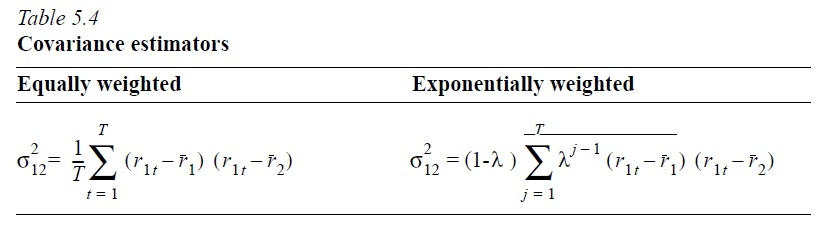
\includegraphics[scale=0.5]{Cov.JPG}

\section{Easy}
\begin{enumerate}
 \item Two coins, one is double tail, you see one \\
  \begin{itemize}
    \item three pancakes: golden-golden, golden-brunt, brunt-brunt, see one golden, probability that the other side is golden two
    \item 
   \end{itemize}
 \item Two coins - one toss n+1, one toss n, probability that n+1 gets more tail than n man?
\end{enumerate}


\section{Medium}
\begin{enumerate}
	\item Use coins to create probabilities : fair coin to create 1/3 probability - toss twice, one result is retoss
unfair coin to create 1/3 probability - combine two toss as one


 \end{enumerate}
 
\chapter{Quantitative Portfolio Mangement}

\chapter{Statistical Arbitrage}

\section{mean-reversion}

intraday mean-reversion

Volatility Clustering and Leverage Effect 

\chapter{Factor Investing}
 
\section{Smart beta and Smart Alpha}                  % Print a "section" heading

long-short STS strategy
short extension( 120/20 ) Strategy
alpha and beta separation
portable alpha 

long short equities (factor) 
convertible arbitrage


\section{Key things to Notice in Index Making}
\section{factor analysis and risk premia}

value, momementum, quality, volatility, betaRM-RF  The return spread between the capitalization weighted stock market and cash.

QUality Minus Junk (quanlity)

SMB      The return spread of small minus large stocks (i.e., the size effect).

HML      The return spread of cheap minus expensive stocks (i.e., the value effect).

RMW     The return spread of the most profitable firms minus the least profitable.

CMA      The return spread of firms that invest conservatively minus aggressively.

UMD (momentum/trend) UMD is long winners and short losers and also from Ken French’s website)

Carry  Vol Carry


Special: liquidity premia 


Market Ineffciency Analysis: funding constraint of financial institutions, grand move of large funds constraints

\section{Market Anomalies}

\subsection{Behavioral Finance}

Behavioral Finance Theories Includes Prospect Theory( People suffice rather than optimize, the utility curve is concave at the gain part and convex at the loss part(loss aversion). Bounded Rationality and 
Behavioral Market Anomalies/bias

\begin{enumerate}
 \item loss aversion(herding)
 \item illusion of control(TAA) 
 \item Mental accounting(goal),
 \item availability bias(familiarity, home-bias)
 \item recency bias(tactical shifts)
 \item framing(risk-return presented in a different way)
\end{enumerate}




other: liquidity risk premia
\begin{enumerate}
 \item Risk Management and Hedging 
 \item Leverage 
 \item Correlation
 \item Strategy replacements, leverage rebalancing and rebalancing frequency, leverage reset
\end{enumerate}


other: liquidity risk premia
\begin{enumerate}
 \item Risk Management and Hedging 
 \item Leverage 
 \item Correlation
 \item Strategy replacements, leverage rebalancing and rebalancing frequency, leverage reset
\end{enumerate}


\chapter{Single (Asset Class) Trading Strategies}
\section{Equity}
\section{Volatility and Dispersion Trades}
	\subsection{Volatility Models and Time-Series Models}
	
\section{fixed income + macro}
\section{fixed income derivatives}

MBS Convexity Trade

    1. real estate-direct vs indirect environment  
    2. benchmarks of real estate
    3. other alternative, commodity to hedge

\section{credit}
\section{commodities} 

\chapter{Quant Strategies and Long-short Strategies}

Stat Arb (typically high volume), Merger Arb, Relative Value, IntraCap Pairs 
 

\part{Quantitative Modeling and Strategies Implementation}

\chapter{Strategy Development Overview}

Typically, need the sub functions/sub teams including:

\begin{enumerate}
 \item Data Curator: Data collection, cleaning, indexing, storing, adjusting and delivering 
 \item Feature Engineering and Analytics: Data Mining, Signal Extraction and Processing using information theory, Data visualization, labeling, filtering, classifiers building - try to extract features
 \item Strategies Research: Make sense of features, market observation, instrument knowledge and try to formulate general theory/intuition that explains market mechanics. Submit code to the backtesting team
 \item Backtesting: Statistical, Stochastic, Econometric tests of strategies/portfolios
 \item Deployment: Rely heavily on computing, process schedulers, automation servers, vectorization, multithreading, multiprocessing, Big Data, Machine Learning on Big Data and High-performance computing 
\end{enumerate}

Also, teams should also maintain and select current strategies, typically, a strategy experiences Embargo, Paper Trading, Real-money trading, Re-allocation and Decommission.

Some Major Challenges:

\begin{enumerate}
 \item Traditional Portfolio Mangers work in silos and make decisions alone. While quant investing need to cut-down the decision making process to small research projects and run as a strategy factor
 \item Combine "black-box" PM views/market intuition with quant research results from data/math. 
 \item Combine machine learning algorithm with existing traditional strategies. 	
 \item "Backtest overfitting": Without limitation on number of trials, Sharpe ratio in back test could be very high. 
\end{enumerate}


\chapter{Financial Data Modeling}

\section{Financial Data Structure}

\section{Financial Data Sampling}

\subsection{Data Sampling Methods}

\subsection{Data Sampling Weights}

\section{Time-series Data Modeling}

\section{Data Labeling in Strategy Research}




\chapter{ Trading System }

\chapter{ Strategy Development Overview}

\section{Strategy Teams}





Data Problems
\begin{itemize}
 \item Bonds: Recall, Termination (Aging), Exchanged
 \item Stock: Corporate Actions (Splits, Reverse Splits, Voting Rights, etc)
 \item Futures and Options: Termination and Rolling
 \item Currencies: Not Traded in centralized order book 
\end{itemize}

Signals

\begin{itemize}
 \item Quote Offers canceling/replacing with sell orders 0 potnetial sell off information
 \item Limit Orders vs Market Orders 
\end{itemize}

\section{ Strategy Development Pipeline(Single/Linear Strategy) }
\subsection{Basic Architecture/System}
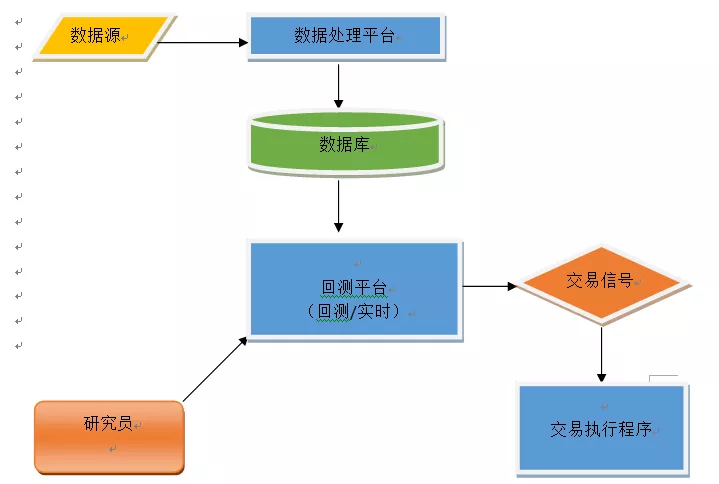
\includegraphics[scale=0.5]{1.JPG}
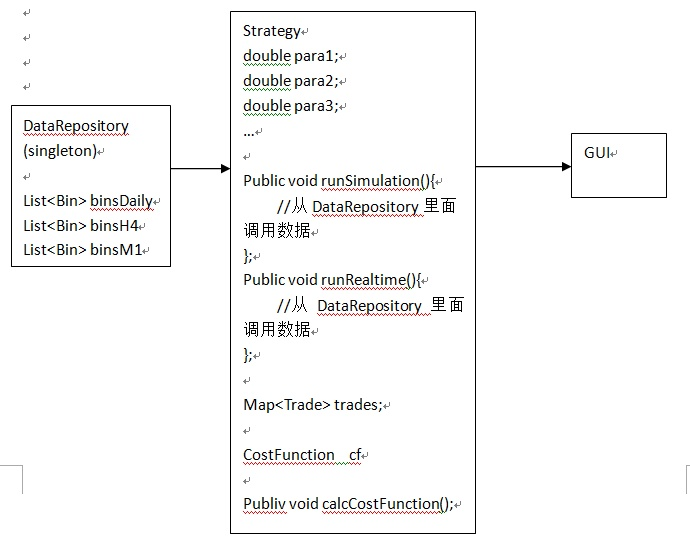
\includegraphics[scale=0.5]{2.JPG}
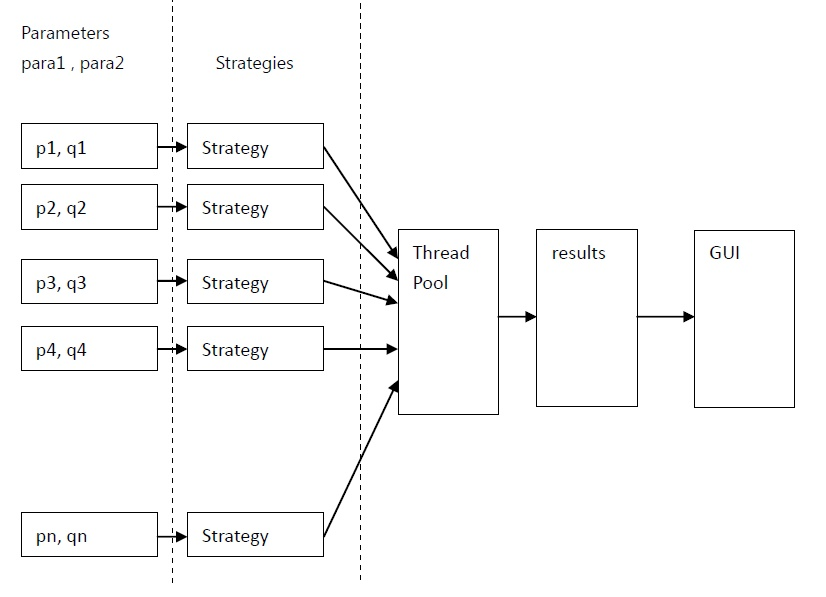
\includegraphics[scale=0.5]{3.JPG}
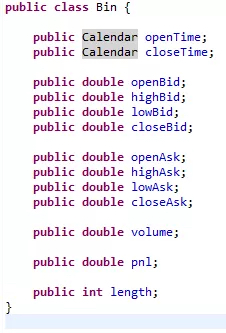
\includegraphics[scale=0.5]{4.JPG}
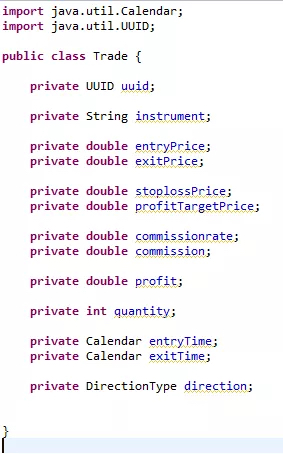
\includegraphics[scale=0.5]{5.JPG}
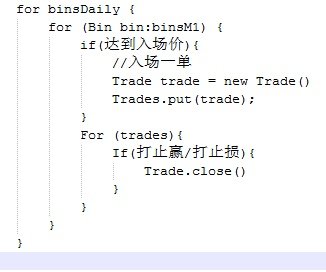
\includegraphics[scale=0.5]{6.JPG}


Historical Data is a singleton. All Market Data (eg. a candle stick ) should be organized to feed the researcher to program strategies on the backtester (eg. like quantopian). All back-testing should be parallized (ideally on GPU) to display parameter-profit relationship. (heatmap, stock charts, etc ) Ideally the optimization process could be visualized (like Tensorflow) 

All like a research facility feedback cycle. 

Key Details: API Design, Module Separation etc. 
\subsection{Data}

Key is a real-time listener. Technical Considerations: KDB, Hadoop and HDFI(?), SQL Like, Mongo Db to store Archive Data. Market Data Providers consideration buying from Wind, BBG, Reuters, Etc. \\

teams: platform operation engineer, analytics builder, strategy control/management and risk management, data team, execution team, researcher team ( 3 x tech )\\

data licensing and data quality insurance \\

data base, text file archive, big data issue\\

cheap data: brokerage: interative brokers.

\subsection{Backtester/Simulator}

Key Components

*Send Singal to Quoting/Trading/Exection Tool(Real Time)
*Market Data Objects (eg. loop for every time bins)
*stop loss/risk control system integration
*parameter-backtest profit/statistics result: optimization and loss function set function to tune the parameters
*multi-thread: Java backter (Java thread pool*)
*human selection of parameters: parameter table and visualization

\subsection{Trade Record and Money Management}

record every trade, summarize execution shortfall, statistical trends and information (shortcomings of strategy executions) and market information ( learning material) build statistics and storage

More: order book and trade book level data handling

\subsection{Analytics}

\subsubsection{ Strategy Management }, Sharpe Anslysis, Holding Period, Slippage visualization to better assistant strategic allocation

\subsubsection{Execution Analysis and Cost}

quantitative trading/systematic trading strategies:
* equity long/short

\subsection{Research Team}
Key problems:
* Optimization and Combination of Sub-Strategies (Eg. factors)
* Market Regime Change Detection(problem not solved): Distinguish between trend and oscillation market
* market supply/demand imbalance analysis (risk-premia) 
* volatility trading, dispersion trading - 2nd and 3rd degree trading, (vol model, vol clustering effect, vol leverage effect)
* hedging/overlay strategy research: hedging cost and hedging risk management, how to adjust hedge according to market condition.
* common ideas: market imbalance, mean-reversion, autocorrelation patterns etc (find patterns and trade) - based on statistics.  Risk factors, implied arbitrage - based on math. 

\subsubsection{Parameter Optmization and Control}

Rely on GUI - parameter distribution and selection
optmization methdologies from machine learning ( see optimization chapter)
robustness anslysis and out-of sample test ** ( random cut the universe of rolling window on selection period )

\subsubsection{Signal Indicator Design}

For example, based on fundemental ratio and technical indicators - design a formula. And check the level of prediction power (if any)

1.seeking stationarity: find a stationary time series
	use difference, integration, and normalize with volatility 
2.find signal level, plot cumulative back-test return against different signal level (use own quotes, and use signal level to filter quotes)
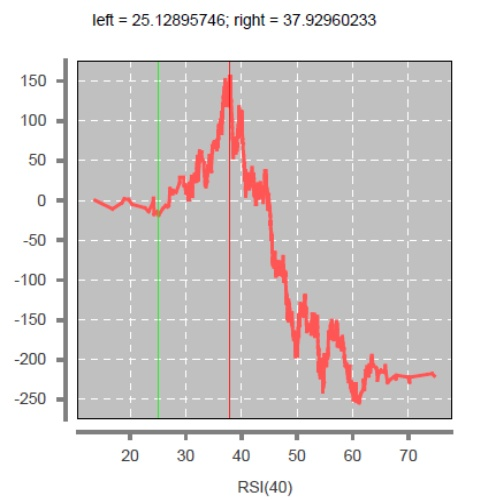
\includegraphics[scale=0.5]{7.JPG}
3.Check stability of customized indicators 
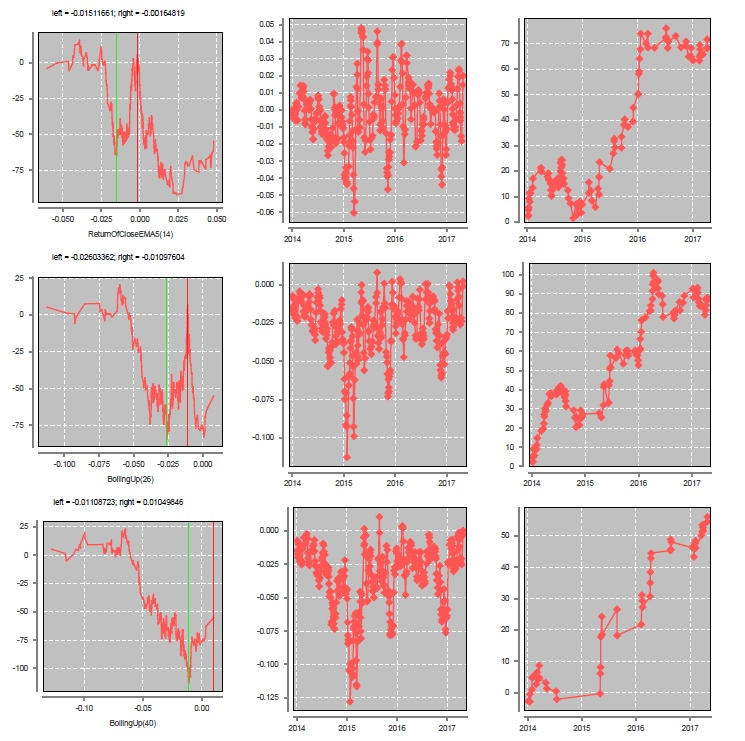
\includegraphics[scale=0.5]{8.JPG}
4. check overfitting and type-II error in all settings, apply noise filtering if possible 
5. design a interface to input indicator(math formula parser to read string) and visualize information using GUI.(HTML/XML Render)
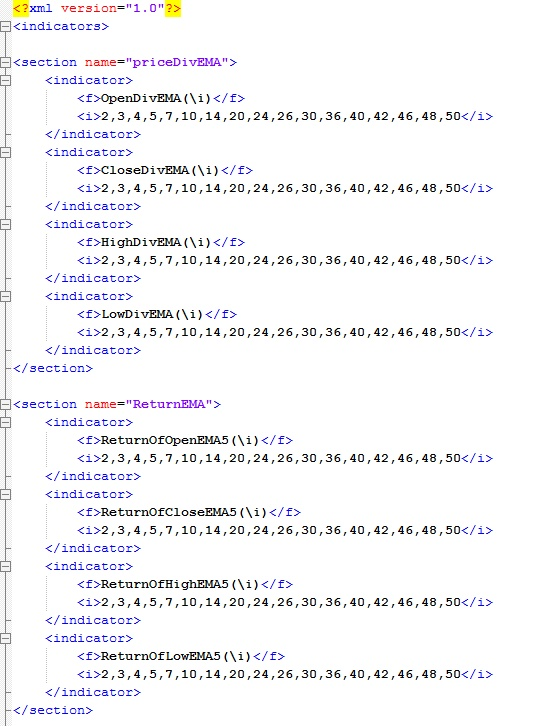
\includegraphics[scale=0.5]{9.JPG}
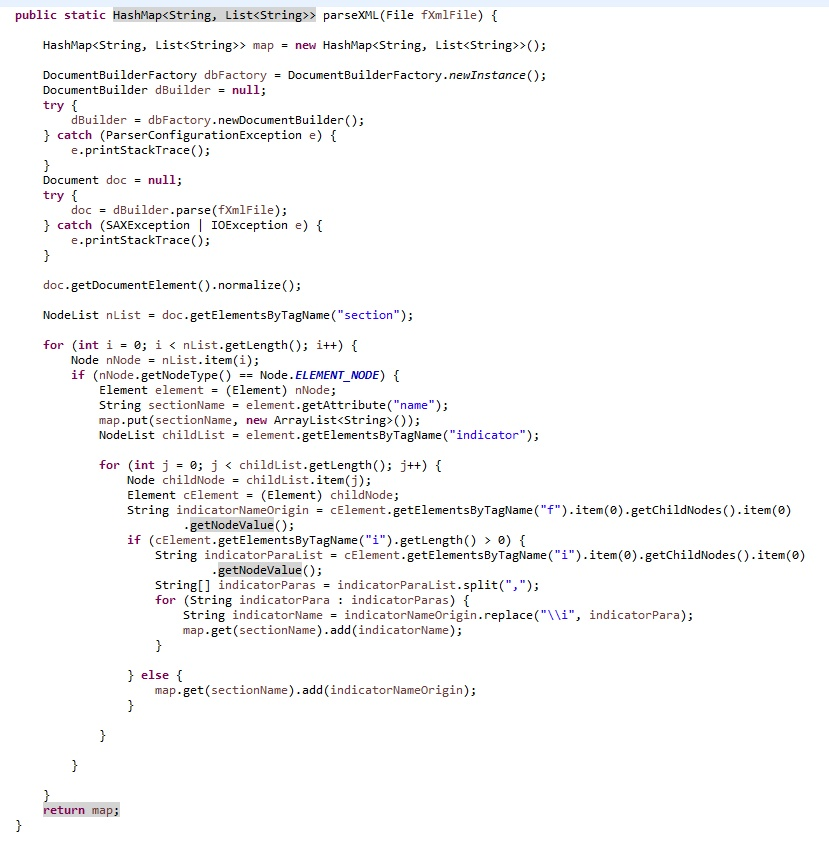
\includegraphics[scale=0.5]{10.JPG}
6. aggregate all indicators( eg. macd, ead ). Aggregate all strategies using optimization framework or selection framework to gain statistical alpha
7. indicator effectiveness test
1. test correlation - the correlation between indicator and profit vs. the correlation between correlation and white noise(hypothesis test) * use spearman correlation rather than pearson correlation* 
2. Use Monte Carlo Simulation to do permutation test of effectiveness of indicator
3. Very very hard - detect sensentivity to market regime change(osicallation and trend) and identify market regime change. 

\subsubsection{Integration of single indicators and portfolio theory}

Form indicator as factors: standardization to mean-0, normal/t-distributed scores. Select powerful ones (ones that passed the permutation test). Optimize to maximize holdings exposure to factor with risk penalty. The key is still feature engineering.

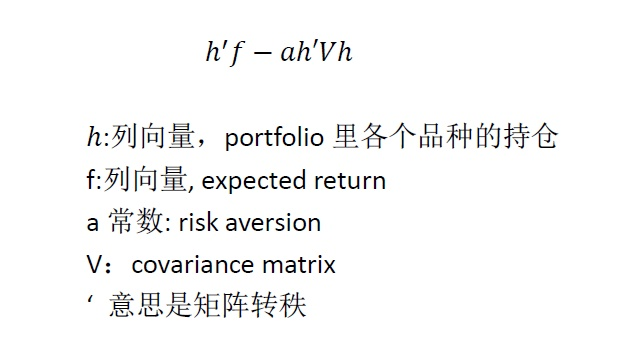
\includegraphics[scale=0.5]{11.JPG}

For Covariance, See section "covariance matrix".  



\subsubsection{Strategy Risk Management and Money management}

small stop loss, big stop gain level on reversion strategies.bigger stop loss, smaller stop gains on volatile markets - based on experience, market analysis.

Choose symmeteric/non-symmetric risk control based on market belief

Hedging and Market Exposture Management - Volatility Control and Automatic de-leveraging. 

together with cost consdieration. 

\section{Backtesting}

\begin{enumerate}
 \item Surviorship-bias
 \item Look ahead-bias
 \item In-sample bias
\end{enumerate}

\chapter{Portfolio Risk Management}

\section{Derivatives and Hedging Strategies}


Sell Side Risk

Coherent  Risk measure

monotonicity

subadditivity

positive homogeneity

translation invariance



liquidity risk


funding liduitdity
market liquidity ( brokerage fees, execution price compared to mid-point, impact of transaction in the market price, the speed of transaction execution)


evidence that liquidity good: stable quoted bid-ask spread, order book depth deep, falling realized bid-ask spread, 
evidence for bad liquidity: large trades have more market impact, average trade size fall, increased bifurcation in the corporate bond market( different liquidity preferring on-the-run)


influncers

regulators( e.g. leverage, Volker Rule)

Central bank
  bank funding channel
  market functioning channel
 risk appetite channel

liquidity measures
bid-ask spread
effective spread
Roll’s price reversal 
Corwin and Schultz high-low spread 
price impact
turnover
Amihud’s measure
Markit’s liquidity score
Dealer count
Quote depth
Imputed round-trip cost






tightness: cost of a round-trip transaction
market depth: how much moved by a large order
resiliency : length of time for which a lumpy order moves the market away from the equilibrium price
adverse price impact
slippage( the amount of deterioration in the market price induced by the amount of time it takes to get a trade done)  


model validation(quantitative)

validation of inputs and parameters(assumptions)
model replication
benchmarking and hypothetical portfolio testing (with another strategy)
backtesting
profit and loss distribution
stress testing\

2. risk management
    1. Var - historical, analytical, MC good and bad
    2. credit risk exposure (pv only swap has)
3. derivatives  
    1. futures, hedge, synthetic equity/cash, pre-investing
    2. options
        1. spread-bull bear, butterfly   
        2. straddle, collar, box spread( bull, bear spread- risk free rate)
        3. interest rate swap - leveraged floating-rate notes, inverse floater; currency swap
        4. swaption - payer, receiver - use receiver to add/remove callable bond features 


1. fixed income
    1. duration matching 
        1. requirements
        2. vs cashflow matching(tenor offer), contingent immunization, horizon matching
    2. index and challenges 
        1. index vs mutual fund,ETF, synthetic strategies(total return swap, less cash but counterparyt risk )
    3. yield curve strategies
        1. laddered, bullet, barbell vs level slope curvature
        2. barbell vs bullet, condor and butterfly long short at level change, slope change, curvature change, yield volatility change performance and strategy (wing and body)
    4. high yield and credit stprad
        1. IGB HYB : credit risk, credit migration risk, interest rate risk, liquidity risk
        2. access liquidity risk and tail risk 
        3. emerging market difference 


\section{FX risk management}
    1. currency management 
        1. forward price (long/short base currency) 
        2. options- risk reversal, put spread, seagull spread
    2. index and benchmark
        1. capitalization-weighted, price-weighted, equal-weighted index, fundamental-weighted indexes 



\chapter{Monitoring and Performance Evaluation}

\section{Monitoring}
    1. rebalancing corridor width
    2. CPPI/ swaption etc

\section{Performance Evaluation}

\subsection{Equity}

Factor Model (Axima, Barra) 
\subsection{Fixed Income}

    1. fixed income - no contribution-risk-free-asset categories-benchmark level(style)-manger-allocation effects(residual) 


\chapter{Alternative Data and General Machine Learning}

\chapter{E-trading and Execution}

Program Trading: Trading a group of instruments, typically cash equities, as single unit (Portfolio Trading or Basket Trading) Commissions from 3bps to 15 bps (2018). Used by active funds, arbitragers (derivatives to cash (eg. Treasury and Treasury Futures)etc)

Hedge Funds use it as part of Stat Arb (typically high volume), Merger Arb, Relative Value, IntraCap Pairs


Execution, Market Impact, VWAP 


\begin{thebibliography}{999}

\bibitem{lamport94}
  Marcos Lopez De Pardo, 
  \emph{Advances in Financial Machine Learning}.
  Wiley,
  1st Edition,
  2018

\end{thebibliography}
 
\end{document}                          % The required last line 